\newpage

\section{Q4}

\begin{figure}[htbp]
    \centering
    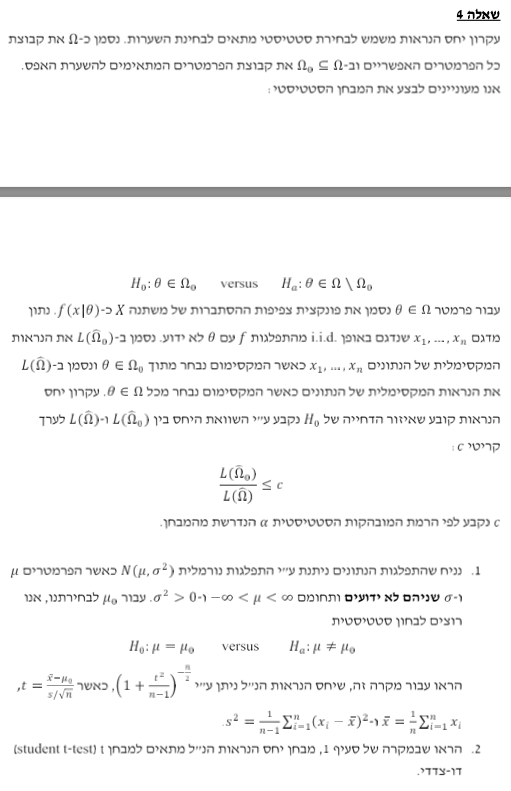
\includegraphics[width=0.65\linewidth]{images/q41.png}
    \caption{q4.1 4.2}
    \label{fig:q4.1}
\end{figure}

\begin{figure}[htbp]
    \centering
    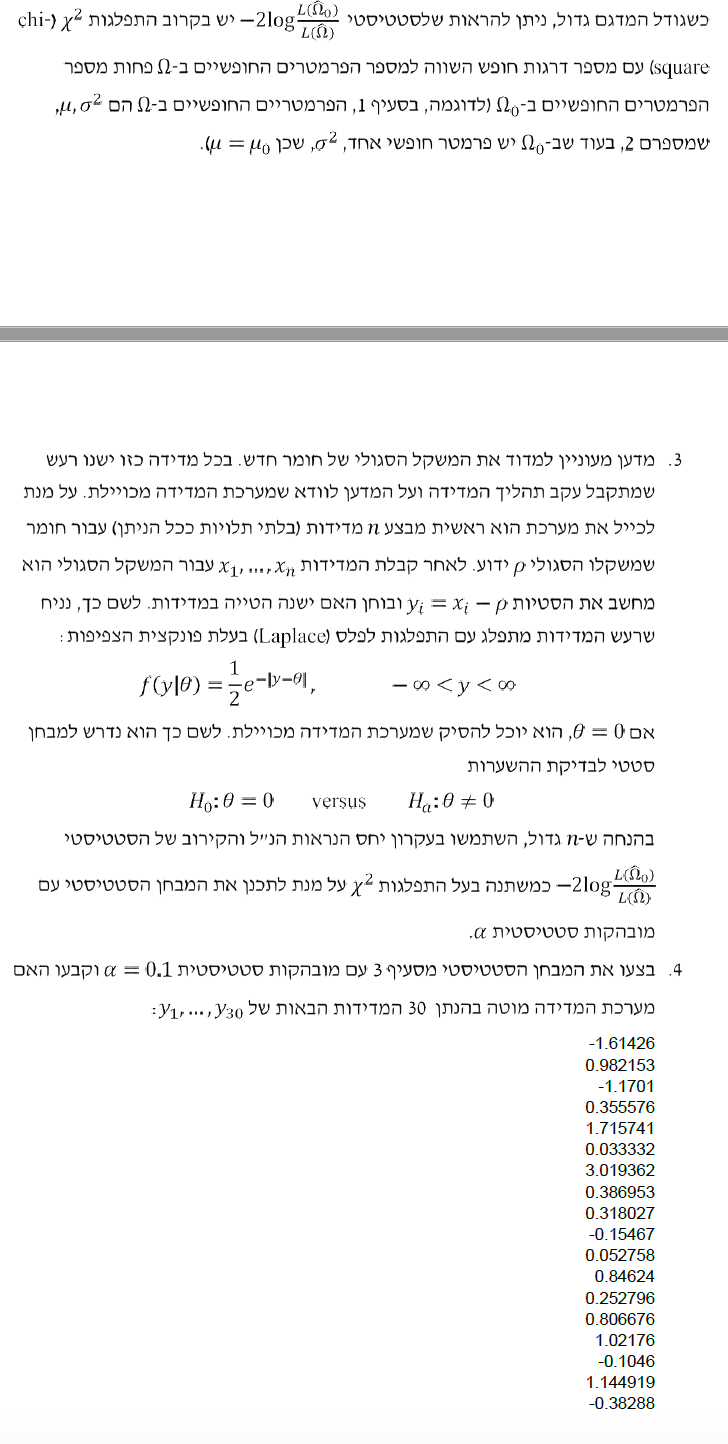
\includegraphics[width=0.65\linewidth]{images/q4.png}
    \caption{q4.3 4.4}
    \label{fig:q4.2}
\end{figure}

\newpage
\subsection{Q4.1}
Given distribution $N(\mu,\sigma^2)$ such that $\mu$ and $\sigma$ 
are both unknown and their range's are $- \infty < \mu < \infty $
and $\sigma^2>0$.
for $\mu_0$ for our choice we want to statistic test:
$H_0 : \mu = \mu_0 $ versus $H_a:\mu \neq \mu_0$

show that for this condition, the likelihood ration is $\left( 1+\frac{t^2}{n-1}\right)^{-\frac{n}{2}} $
given that:
$t=\frac{\overline{x}-\mu_0}{s/\sqrt{n}}$ and
$\overline{x}=\frac{1}{n}\Sigma^{n}_{i=1}x_i$ and
$s^2=\frac{1}{n-1}\Sigma^{n}_{i=1} \left(x_i - \overline{x} \right)^2$ \\

\textbf{Solution:}

First, lets calculate the maximum likelihood estimate (MLE) for the variance $\sigma^2$ for $H_0$ for normal distribution, the likelihood is:

\[ L(\sigma^2) = \prod_{i=1}^{n} \frac{1}{\sqrt{2\pi\sigma^2}} \exp\left(-\frac{(X_i - \mu)^2}{2\sigma^2}\right) \]

The likelihood with log is easier to work with is:

\[ \ln L(\sigma^2) = \sum_{i=1}^{n} \left[ -\frac{1}{2} \ln(2\pi) - \frac{1}{2} \ln(\sigma^2) - \frac{(X_i - \mu)^2}{2\sigma^2} \right] \]

Now when we are differentiating the likelihood with log function with respect to $\sigma^2$ and set it to 0:

\[ \frac{d}{d\sigma^2} \ln L(\sigma^2) = \sum_{i=1}^{n} \left[ -\frac{1}{2\sigma^2} + \frac{(X_i - \mu)^2}{2(\sigma^2)^2} \right] = 0 \]

Lets solve for $\sigma^2$

\[ \hat{\sigma}^2 = \frac{1}{n} \sum_{i=1}^{n} (X_i - \mu)^2 \]

This is the MLE of the variance for $H_0$.

For $H_a$,there are two unknown parameters for calculating the MLE: 

\[ \ln L(\mu, \sigma^2) = -\frac{n}{2} \ln(2\pi) - \frac{n}{2} \ln(\sigma^2) - \frac{1}{2\sigma^2} \sum_{i=1}^{n} (X_i - \mu)^2 \]

Taking the partial derivative with respect to $\mu$ and setting it to zero,

\[ \frac{\partial}{\partial \mu} \ln L(\mu, \sigma^2) = \frac{1}{\sigma^2} \sum_{i=1}^{n} (X_i - \mu) = 0 \]

gives the MLE of $\mu$,

\[ \hat{\mu} = \frac{1}{n} \sum_{i=1}^{n} X_i \]

Similarly, differentiating with respect to $\sigma^2$ and setting to zero,

\[ \frac{\partial}{\partial \sigma^2} \ln L(\mu, \sigma^2) = -\frac{n}{2\sigma^2} + \frac{1}{2(\sigma^2)^2} \sum_{i=1}^{n} (X_i - \mu)^2 = 0 \]

provides the MLE of $\sigma^2$,

\[ \hat{\sigma}^2 = \frac{1}{n} \sum_{i=1}^{n} (X_i - \hat{\mu})^2 \]

These are the maximum likelihood estimates of $\mu$ and $\sigma^2$ 

Given the $t$-statistic, sample mean $\overline{x}$, and sample variance $s^2$ defined as:
\begin{align*}
t &= \frac{\overline{x} - \mu_0}{s/\sqrt{n}}, \\
\overline{x} &= \frac{1}{n}\sum_{i=1}^{n} x_i, \\
s^2 &= \frac{1}{n-1}\sum_{i=1}^{n} (x_i - \overline{x})^2,
\end{align*}
we aim to show that the likelihood ratio, $\Lambda$, under certain conditions, is:
\[ \Lambda = \left( 1+\frac{t^2}{n-1}\right)^{-\frac{n}{2}}. \]

\[ \Lambda = \frac{L(H_0)}{L(H_a)}. \]

\[ \Lambda = \left( 1+\frac{t^2}{n-1}\right)^{-\frac{n}{2}} \]




\subsection{Q4.2}

\subsection{Q4.3}

\subsection{Q4.4}